%% ============================================================
%%  Chapter 5 — Perovskite Semiconductor Radiation Detectors
%%  Dissertation: Radiation Responsive Materials for Advanced
%%  Radiation Detection and Systems
%% ============================================================

\chapter{Perovskite Semiconductor Radiation Detectors}
\label{ch:perovskite_detectors}

The preceding chapter established that photovoltaic-architecture
perovskite thin films can generate measurable current-mode signals
in response to X-ray, gamma, and neutron irradiation, exploiting
the device's built-in electric field to sweep radiation-generated
carriers to the contacts without any externally applied bias.  The
present chapter pursues a fundamentally different detection
philosophy: deploying thick single-crystal halide perovskites as
direct-conversion semiconductor radiation detectors in which a
large externally applied reverse bias sweeps charge carriers
generated by individual radiation interaction events across the
bulk crystal and into a charge-sensitive readout chain.  This mode
of operation, familiar from conventional compound semiconductor
detectors such as CdZnTe (CZT) and Cd\-Te, offers the possibility of
pulse-by-pulse energy spectroscopy rather than the integrated
current monitoring that characterises the photovoltaic geometry
of Chapter~\ref{ch:CsFAPbI}.

Halide perovskites present a compelling case for direct-conversion
detector development.  Their heavy-metal cation sublattice —
dominated by lead in the systems studied here — provides a high
effective atomic number, giving large photoelectric cross sections
at gamma and X-ray energies that are difficult or impossible to
achieve with silicon or organic semiconductors.  Some
methylammonium-based and methylhydrazinium-based compositions
additionally incorporate a high density of hydrogen atoms, enabling
elastic proton-recoil reactions with fast neutrons that allow
direct-conversion neutron detection without requiring a separate
conversion layer.  Solution-phase crystal growth methods developed
over the past decade for photovoltaic research have produced
centimetre-scale single crystals with carrier $\mu\tau$ products
approaching or exceeding those of polycrystalline CZT, a property
critical for efficient charge collection across the millimetre-scale
thicknesses required to stop MeV-energy photons and neutrons.

The experimental program described in this chapter spans three
perovskite crystal chemistries and three radiation types.
MAPbI$_3$ crystals doped with hexagonal boron nitride (hBN),
referred to here as MAPbI$_3$-hBN, were characterised as X-ray
detectors over an extended range of applied bias voltages,
including tests under vacuum to isolate the role of atmospheric
humidity (Section~\ref{sec:xray_detector}).  A family of bromide
perovskites — CsPbBr$_3$, MAPbBr$_3$, and FAPbBr$_3$ — was
developed as gamma-ray spectrometers, with the Cs-137 and Co-57
photopeak measurements reported in
Section~\ref{sec:gamma_detector}.  The novel organic-metal halide
perovskite MHyPbCl$_3$ (methylhydrazinium lead trichloride) was
synthesised and tested as a fast neutron detector using the Fast
Beam Facility (FBF) at the Ohio State University Research Reactor,
with results presented in Section~\ref{sec:neutron_detector}.
Throughout all three of these application domains, a recurring
materials-physics challenge — the migration of halide ions under
the large electric fields required for efficient charge collection
— dominated the device performance and ultimately set the practical
limits on applied bias, detector lifetime, and energy resolution.
Section~\ref{sec:ion_migration_detector} analyses ion migration in
detail and discusses the mitigation strategies evaluated in this
work.


%% ------------------------------------------------------------
\section{Perovskite Semiconductor Detector Principles}
\label{sec:detector_principles}
%% ------------------------------------------------------------

A direct-conversion radiation detector converts the energy deposited
by an ionising particle or photon directly into an electrical signal,
without an intermediate scintillation step.  When a gamma ray,
X-ray, or charged particle deposits energy $E$ in a semiconductor
detector of bandgap $E_g$, approximately $E/W$ electron-hole pairs
are created, where $W \approx 2.8\,E_g$ is the mean ionisation
energy per pair~\cite{knoll2010}.  The carriers are swept by an
applied electric field to opposite contacts, where they induce a
charge pulse on the readout electronics.  For spectroscopic
operation, this pulse must be faithfully proportional to the
deposited energy — a condition that requires complete charge
collection and minimal trapping of carriers en route to the contacts.

The probability that a carrier generated at depth $x$ in the
crystal (of thickness $d$) reaches the collecting contact is
described by the Hecht equation,

\begin{equation}
  \eta = \frac{\mu\tau E}{d}
    \left[1 - \exp\!\left(-\frac{d}{\mu\tau E}\right)\right],
  \label{eq:hecht}
\end{equation}

\noindent where $E = V/d$ is the applied electric field,
$V$ is the applied voltage, and $\mu\tau$ is the
mobility-lifetime product of the carrier species (electrons
or holes) that dominates collection~\cite{Hofstadter1949}.
Equation~(\ref{eq:hecht}) shows that achieving high collection
efficiency $\eta \to 1$ requires either a large $\mu\tau$
product or a large applied field, or both.  For a 1-mm-thick
crystal with $\mu\tau = 10^{-3}$~cm$^2$\,V$^{-1}$, for
instance, complete collection requires fields of order
10~V\,$\mu$m$^{-1}$, i.e.\ applied voltages of order 1~kV.
This requirement for large applied voltages is in direct
tension with the ion-migration instability described in
Section~\ref{sec:ion_migration_detector}.

Two additional material requirements govern detector performance.
First, the dark resistivity $\rho$ must be sufficiently high that
the leakage current $I_{\rm dark} = V\!A/(\rho d)$ (where $A$ is
the contact area) produces an electronic noise contribution smaller
than the signal charge from the smallest radiation event of interest.
For gamma spectroscopy with CZT-like performance, $\rho > 10^{9}$~$\Omega$\,cm
is typically required~\cite{Luke1995}.  The three-dimensional
(3D) halide perovskites studied in this work achieve resistivities
in the range $10^{9}$--$10^{12}$~$\Omega$\,cm in their highest-quality
single-crystal forms, competitive with or exceeding that of
polycrystalline CZT.  Second, the crystal must be thick enough
to stop a significant fraction of the incident radiation.  The
mean free path of a 662-keV gamma ray (the primary emission of
$^{137}$Cs) in CsPbBr$_3$ is approximately 7~mm, meaning that
crystals of order 5--10~mm are required for reasonable detection
efficiency.  Growing defect-free perovskite single crystals at
these length scales presents a significant fabrication challenge,
discussed in Section~\ref{sec:fabrication}.

For fast neutron detection, the governing interaction is not
photoelectric absorption but elastic proton recoil: a fast neutron
of kinetic energy $E_n$ collides with a hydrogen nucleus
(proton), transferring up to $E_n$ of kinetic energy to the recoil
proton in a head-on collision.  The recoil proton then deposits
its energy densely in the crystal volume, generating a large
number of electron-hole pairs.  The detection efficiency of a
hydrogenous material is therefore proportional to its hydrogen
atom density $n_H$.  Table~\ref{tab:h_density} compares $n_H$
for the key materials considered in this work.

\begin{table}[htbp]
\centering
\caption{Hydrogen atom density comparison for fast neutron
         detector materials.  MHyPbCl$_3$ achieves a hydrogen
         density comparable to organic scintillators despite
         being an inorganic-organic hybrid perovskite.}
\label{tab:h_density}
\begin{tabular}{lllc}
\hline
Material & Formula & Density (g\,cm$^{-3}$) & $n_H$ (cm$^{-3}$) \\
\hline
Stilbene          & C$_{14}$H$_{12}$  & 1.16 & $5.67\times10^{22}$ \\
Rubrene           & C$_{42}$H$_{28}$  & 1.27 & $3.62\times10^{22}$ \\
EJ-276 plastic    & C$_n$H$_m$        & 1.02 & $4.82\times10^{22}$ \\
MHyPbCl$_3$       & CH$_6$N$_2$PbCl$_3$ & 3.25 & $\sim4.0\times10^{22}$ \\
\hline
\end{tabular}
\end{table}


%% ------------------------------------------------------------
\section{Materials, Crystal Growth, and Device Fabrication}
\label{sec:fabrication}
%% ------------------------------------------------------------

\subsection{Perovskite Crystal Systems}
\label{sec:crystal_systems}

Four distinct halide perovskite crystal chemistries were
investigated as detector platforms.
MAPbI$_3$ doped with hexagonal boron nitride
(hBN) was used as an X-ray detector medium.  The hBN
inclusions were incorporated to improve grain boundary
passivation and reduce the density of deep-level trap states
that would otherwise act as recombination centres for
radiation-generated carriers.  The 3D bromide perovskites
CsPbBr$_3$, MAPbBr$_3$, and FAPbBr$_3$ — where Cs, MA, and
FA denote the inorganic caesium, methylammonium, and
formamidinium A-site cations, respectively — were pursued as
gamma-ray spectrometers on account of their wide bandgap
($\sim$2.3~eV), which provides the high dark resistivity
essential for low-noise spectroscopy, their large effective
atomic number driven by the Pb and Br sublattices, and
their excellent carrier transport properties demonstrated
in the photovoltaic literature~\cite{Saidaminov2015,He2019CsPbBr}.
Finally, MHyPbCl$_3$ (methylhydrazinium lead trichloride),
where MHy denotes the CH$_3$NH$_2$NH$_2^+$ methylhydrazinium
cation, was selected as a fast neutron converter on the basis
of its high hydrogen density, which places it on a par with
conventional organic fast-neutron scintillators
(Table~\ref{tab:h_density}), combined with the direct
charge-collection advantage of a semiconductor~\cite{Panaccione_NIM_2024}.

\subsection{Crystal Growth Procedures}
\label{sec:crystal_growth}

\subsubsection{MHyPbCl$_3$ Synthesis}

Methylhydrazinium chloride (MHyCl) was first synthesised as the
organic precursor salt.  To obtain MHyCl, 2.63~mL (50~mmol)
of methylhydrazine was diluted with 5~mL of anhydrous
isopropanol (IPA), and 100~mL of 0.5~M HCl solution was added
to the IPA mixture without stirring.  After the combined
solution was stored overnight in an inert atmosphere at room
temperature, white plate crystals of MHyCl precipitated
spontaneously.  The crystals were filtered, washed with cold
IPA, and dried under vacuum at room temperature, yielding
3.10~g ($\sim$38\%).

Single crystals of MHyPbCl$_3$ were subsequently grown using
an anti-solvent assisted crystallisation method.  Two millimoles
each of MHyCl and PbCl$_2$ were dissolved in a co-solvent mixture
of 5~mL DMF and 1~mL DMSO.  After stirring for 3~h, the
solution was filtered through a 0.22-$\mu$m syringe filter to
remove undissolved particles, then transferred to a 20-mL vial.
This vial was placed inside a 100-mL bottle containing 15~mL
of toluene as the anti-solvent and sealed in a glovebox.  After
one week at room temperature, several clear hexagonal
MHyPbCl$_3$ crystals formed.  The crystals were harvested
and dried under vacuum.  Immediately prior to electrode
deposition, the crystal surfaces were polished with polishing
paper to remove the polycrystalline surface layer that
accumulates during growth.

\subsubsection{Bromide Perovskite Crystals}

CsPbBr$_3$, MAPbBr$_3$, and FAPbBr$_3$ single crystals
were grown externally and received by the research group
for detector fabrication.  Upon receipt, all crystals were
inspected under optical magnification for internal cracks,
inclusions, and colour uniformity.  Crystals judged to be
free of macroscopic defects were then mechanically planarised
using silicon carbide abrasive paper, followed by sequential
mechanical polishing with diamond polishing paste down to a
10-nm grain size.  The crystals were rinsed with a hexane bath
between each polishing stage to remove residual abrasive
particles.  The final polished faces were inspected for
surface uniformity and flatness prior to contact deposition.
One FAPbBr$_3$ crystal cracked during the polishing stage
and was excluded from subsequent electrical testing; a
bare CsPbBr$_3$ crystal sustained internal cracking from
an accidental drop during handling, and while it remained
electrically functional, the crack likely introduced additional
carrier trapping sites and reduced the geometric solid-angle
efficiency for spectroscopy measurements.

\subsection{Contact Architecture and Deposition}
\label{sec:contact_deposition}

Two distinct contact architectures were used, reflecting
the different electronic requirements of the ohmic and
rectifying contact geometries.

\subsubsection{MHyPbCl$_3$ Ohmic Contact Device}

For the MHyPbCl$_3$ fast neutron detector, an ohmic-ohmic
contact configuration was adopted.  On the lower face of
the crystal, an electron-transport bilayer consisting of
30~nm of C$_{60}$ (fullerene) and 6~nm of bathocuproine
(BCP) was deposited, followed by an 80-nm Cu top layer
to complete the lower ohmic contact.  The upper face of
the crystal received a 50-nm Au contact deposited by
thermal evaporation.  The C$_{60}$/BCP bilayer serves
simultaneously as an electron-selective interlayer and
as a buffer that reduces the density of interface states
at the Cu-perovskite junction.  Current-voltage
characterisation confirmed ohmic, symmetric behaviour
under both polarities of applied bias, consistent with
the intended ohmic-ohmic device architecture.

\subsubsection{Bromide Perovskite Schottky Devices}

For the bromide perovskite gamma detectors, a Schottky
(rectifying) contact architecture was pursued in order
to create a depletion region that would both reduce the
dark current and define the active detection volume of the
device.  A pixelated contact geometry was used, with a
$2\times2$ array of 1.25-mm-diameter titanium pixel contacts
surrounded by an integrated guard ring to intercept and
divert surface leakage currents away from the individual
pixel measurement channels.  On the ohmic side of each
crystal, a 50-nm gold layer was deposited by sputtering.

The Ti Schottky contacts were deposited using an AJA Orion
RF/DC sputter deposition system.  A shadow mask was drilled
from an aluminium sheet to define the pixel and guard-ring
geometry.  The titanium was deposited at 450~W with a
deposition rate of approximately 1.15~\AA\,s$^{-1}$, followed
immediately by a 10-nm nickel passivating overlayer at
250~W (rate $\approx$2.1~\AA\,s$^{-1}$) to prevent
atmospheric oxidation of the titanium surface upon venting.
The gold ohmic contact was deposited on the opposite crystal
face with a Denton sputter coater at a rate of
$\sim$100~\AA\,per 90~s.  Electrical connection was made to
each pixel contact using copper wire leads bonded with
silver epoxy, and the assembled device was mounted in a
shielded enclosure for electrical characterisation.


%% ------------------------------------------------------------
\section{Electrical Characterisation}
\label{sec:electrical_char}
%% ------------------------------------------------------------

\subsection{Resistivity and Dark Current Stability}
\label{sec:resistivity}

Current-voltage (IV) characteristics for all devices were
measured using a Keithley 2612A SourceMeter.  Sweep protocols
ranged from the low-voltage regime ($\pm$2~V at a logarithmic
current resolution of $10^{-12}$~A to confirm ohmic
behaviour and extract contact resistance) to high-voltage
unipolar sweeps (0 to $-100$~V or 0 to $-200$~V) for
resistivity extraction and leakage current characterisation
under detector operating conditions.  All sweeps were
performed with the device in a light-tight enclosure to
prevent photogenerated carrier contributions.

The MHyPbCl$_3$ crystal yielded a resistivity of
$4.43 \times 10^{11}$~$\Omega$\,cm, extracted from the
slope of the ohmic low-field IV characteristic.  This
value places MHyPbCl$_3$ squarely in the range required
for high-sensitivity radiation detectors and exceeds the
resistivity of commercial polycrystalline CZT by roughly
two orders of magnitude, reflecting the low intrinsic
carrier density achievable in high-quality perovskite
single crystals.  The CsPbBr$_3$ device exhibited a
working leakage current in the range of 315--710~nA at
1000~V reverse bias.  This current was not stable upon
first application of bias: the leakage overshot its
quasi-steady-state value immediately after the voltage
was stepped, then decayed gradually over a period of
45~minutes to one hour before approaching a more slowly
varying baseline.  The overshooting behaviour is
consistent with rapid redistribution of mobile halide
vacancies upon application of the field, followed by
slower re-equilibration of the resulting space-charge
distribution.  The FAPbBr$_3$ device demonstrated
substantially lower leakage under high-voltage operation,
with a maximum leakage current of $5 \pm 2.5$~nA during
continuous operation above 700~V, and showed no signs
of electrical instability over more than five hours of
sustained high-voltage testing.

IV hysteresis measurements — sweeping the bias from
forward to reverse and immediately back to forward at a
scan rate of 20~mV\,s$^{-1}$ — served as a sensitive
diagnostic for ion-migration-driven charge redistribution.
The MHyPbCl$_3$ device exhibited a measurable sweep-versus-hold
difference in the low-voltage regime, indicative of a
polarisation effect driven by slow ionic relaxation.
For the bromide perovskites, hysteresis was observed at
all bias levels and was most pronounced at elevated bias,
consistent with field-driven amplification of the
ion-migration rate~\cite{Yuan2016ionmig}.  The mechanistic
origins of this hysteresis and its consequences for
detector operation are examined in detail in
Section~\ref{sec:ion_migration_detector}.

\subsection{Mobility-Lifetime Product}
\label{sec:mut_product}

The $\mu\tau$ product was extracted from photocurrent
measurements under X-ray excitation as a function of
applied bias, fitting the resulting data to
Equation~(\ref{eq:hecht}).  For MHyPbCl$_3$, this
procedure yielded $\mu\tau = 9.1 \times 10^{-3}$~cm$^2$\,V$^{-1}$,
a value comparable to that reported for high-quality
CsPbBr$_3$ single crystals in the
literature~\cite{He2019CsPbBr} and approximately an
order of magnitude larger than typical values for
polycrystalline CZT radiation detector grade material.
The high $\mu\tau$ of MHyPbCl$_3$ indicates that
carriers generated by neutron-induced proton recoil events
can traverse centimetre-scale crystal thicknesses without
significant trapping losses, provided the applied electric
field is sufficiently large.  Physically, the large $\mu\tau$
reflects the extended carrier diffusion lengths achievable
in defect-lean single crystals grown by the anti-solvent
method, where the slow precipitation kinetics produce
crystals with lower intrinsic vacancy concentrations than
those formed by faster-nucleation techniques.


%% ------------------------------------------------------------
\section{X-Ray Detection}
\label{sec:xray_detector}
%% ------------------------------------------------------------

\subsection{Experimental Setup and Dosimetry Calibration}
\label{sec:xray_setup}

X-ray characterisation was performed using a benchtop X-ray
tube operated at tube voltages of 30--50~kVp.  The tube
output was collimated to a conical beam with an exit
aperture of approximately 2~cm at the tube port.  The
primary detector under X-ray evaluation in this chapter
is the MAPbI$_3$-hBN device.  The photocurrent induced by
X-ray exposure was measured as a function of applied bias
using the Keithley 2612A SourceMeter, with the X-ray
beam switched on and off periodically to distinguish the
radiation-induced signal above the dark-current baseline.
The X-ray sensitivity $S$ is defined as

\begin{equation}
  S = \frac{\Delta I}{A \cdot \dot{D}},
  \label{eq:sensitivity}
\end{equation}

\noindent where $\Delta I$ is the X-ray-induced change
in current, $A$ is the active contact area, and
$\dot{D}$ is the X-ray dose rate incident on the detector.
The dose rate was calibrated using a RaySafe 452 dosimeter
positioned in the beam.  The RaySafe 452 contains 24 silicon
diodes and one Geiger-Müller tube distributed over a large
active area, which introduced a systematic calibration
uncertainty when the detector active area was smaller than
the dosimeter sensing region.  In particular, the conical
beam geometry caused the dose rate to vary across the dosimeter
face, leading to an underestimation of the dose rate
incident on the small perovskite contact area.  To address
this, NanoDot optically stimulated luminescence (OSL)
dosimeters — which integrate dose over a localised area
comparable to the perovskite contact dimensions — were
identified as a more appropriate calibration tool for
subsequent experiments.

\subsection{X-Ray Sensitivity of the MAPbI$_3$-hBN Detector}
\label{sec:xray_sensitivity}

Figure~\ref{fig:xray_sensitivity} shows the extracted
X-ray sensitivity of the MAPbI$_3$-hBN device as a
function of applied bias voltage.  At 5~V reverse bias
the sensitivity was $0.107~\mu$C\,(Gy\,cm$^2$)$^{-1}$.
Increasing the bias to 10~V raised the sensitivity to
a measured mean of
$0.245~\mu$C\,(Gy\,cm$^2$)$^{-1}$ (two independent
measurements yielding 0.245 and 0.252~$\mu$C\,(Gy\,cm$^2$)$^{-1}$
at the same bias, confirming reproducibility), and at
20~V the sensitivity reached
$0.411~\mu$C\,(Gy\,cm$^2$)$^{-1}$.  The monotonic
increase of sensitivity with applied bias is consistent
with Equation~(\ref{eq:hecht}): as the electric field
increases, the carrier drift length grows, fewer carriers
are trapped before reaching the contacts, and the
collected charge per unit deposited energy increases
correspondingly.  The sub-linear growth of sensitivity
with voltage — a factor of $\sim$3.8 increase in
sensitivity for a factor of four increase in voltage —
suggests that the device has not yet entered the
charge-collection saturation regime at 20~V, and that
further gains could be achieved at higher fields.

\begin{table}[htbp]
\centering
\caption{X-ray sensitivity of the MAPbI$_3$-hBN detector
         as a function of applied bias.  Sensitivity values
         are extracted from the ratio of the X-ray-induced
         current to the calibrated dose rate multiplied by
         the contact area (Equation~\ref{eq:sensitivity}).}
\label{tab:xray_sensitivity}
\begin{tabular}{cc}
\hline
Applied Bias (V) & Sensitivity ($\mu$C\,(Gy\,cm$^2$)$^{-1}$) \\
\hline
5  & 0.107 \\
10 & 0.245 \\
10 & 0.252 \\
20 & 0.411 \\
\hline
\end{tabular}
\end{table}

\begin{figure}[htbp]
  \centering
  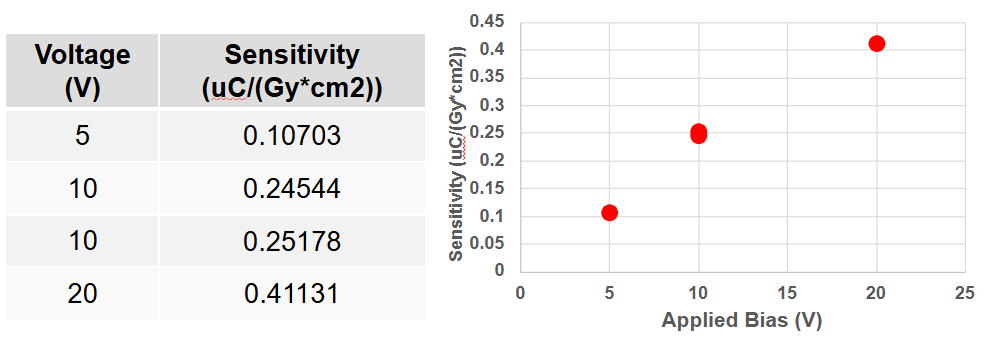
\includegraphics[width=0.65\textwidth]{figures/5_1_xray_sensitivity}
  \caption{X-ray sensitivity of the MAPbI$_3$-hBN detector
           as a function of applied reverse bias.  Sensitivity
           increases monotonically with field, consistent with
           improved charge collection efficiency described by
           the Hecht equation (Equation~\ref{eq:hecht}).
           Error bars represent the spread between repeated
           measurements at the same bias condition.}
  \label{fig:xray_sensitivity}
\end{figure}

The absolute sensitivity values measured here —
of order $10^{-1}$~$\mu$C\,(Gy\,cm$^2$)$^{-1}$ at
modest bias voltages — are substantially below those
reported for optimised 2D perovskite thin-film
detectors.  Tsai et al.\ demonstrated sensitivities
approaching $1000~\mu$C\,(Gy$_{\rm air}$\,cm$^2$)$^{-1}$
in 2D (PEA$_2$MA$_2$Pb$_3$I$_{10}$) detectors at
$-4$~V bias after surface treatment with a
fluorinated phenylethylammonium iodide (5F-PEAI) layer,
and $\sim$828~$\mu$C\,(Gy$_{\rm air}$\,cm$^2$)$^{-1}$
without treatment~\cite{Tsai2022ionmig}.  The gap between
these values and those measured for MAPbI$_3$-hBN
reflects several differences: the 2D perovskite geometry
benefits from a much thinner absorber layer (approximately
9~$\mu$m) that charges and discharges rapidly under the
applied field, while the thick 3D crystal under study here
requires much larger absolute voltages to achieve
equivalent electric fields.  This comparison motivates
the use of higher bias voltages in future 3D crystal
experiments, provided that ion migration can be sufficiently
suppressed to avoid device failure.

A bi-polar X-ray response was observed at zero applied
bias in some MAPbI$_3$-hBN device configurations, wherein
a spontaneous photovoltaic-like current transient was
generated by X-ray exposure without any external voltage
source.  This response is attributed to the asymmetric
contact architecture, which creates a built-in potential
difference between the hBN/MAPbI$_3$ and the Au contact
interfaces.  The built-in field sweeps radiation-generated
carriers toward the respective contacts even in the absence
of applied bias, producing a net photocurrent that switches
polarity depending on the direction of the dominant carrier
flow.

\subsection{Vacuum Testing and Humidity Effects}
\label{sec:vacuum_testing}

The role of atmospheric humidity in X-ray detector performance
was directly evaluated by repeating X-ray sensitivity
measurements on the MAPbI$_3$-hBN device under vacuum
conditions (base pressure $< 10^{-3}$~Torr) and comparing
the results to measurements performed in ambient laboratory
air.  Figures~\ref{fig:vacuum_5v}--\ref{fig:vacuum_20v}
present the X-ray current transients at 5, 10, and 20~V
applied bias under both conditions.  In each case, the
X-ray-induced current was larger and more stable under
vacuum than under ambient atmosphere at matched bias, and
the dark-current baseline was lower under vacuum.  These
improvements are consistent with the suppression of
moisture-accelerated ion migration under vacuum.  When
water molecules are present at grain boundaries and crystal
surfaces, they facilitate the diffusion of halide vacancies
under the applied field, creating shunting pathways and
broadening the internal electric field distribution in ways
that reduce the effective field in the bulk and hence the
charge collection efficiency.  Removal of ambient moisture
under vacuum disrupts this pathway and partially restores
the intrinsic carrier transport properties of the crystal.

\begin{figure}[htbp]
  \centering
  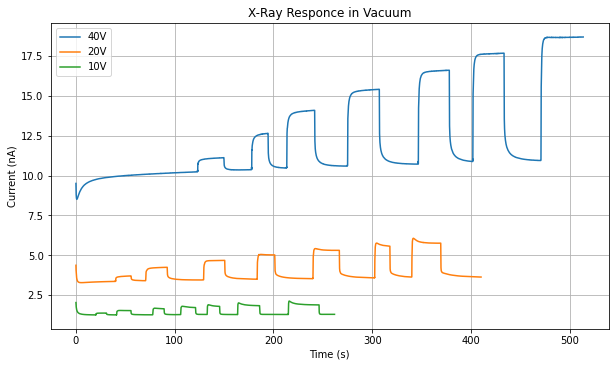
\includegraphics[width=0.80\textwidth]{figures/5_2_vacuum_comparison}
  \caption{Comparison of X-ray current transients at 5, 10,
           and 20~V applied bias for the MAPbI$_3$-hBN device
           in ambient air (solid curves) and under vacuum
           (dashed curves).  Vacuum operation consistently
           produces a larger and more stable radiation-induced
           current, attributed to suppression of
           moisture-accelerated ion migration.}
  \label{fig:vacuum_comparison}
\end{figure}

Despite the improvements afforded by vacuum operation, the
MAPbI$_3$-hBN device ultimately failed after approximately
five hours of continuous operation at 400~V applied bias.
Post-failure inspection showed that the device could no
longer sustain any significant reverse bias, consistent
with the formation of a low-resistance shunting pathway
through the crystal bulk.  This failure mode — also
documented by Tsai et al.\ for 2D perovskite detectors
operating above their breakdown threshold — is attributed
to the catastrophic redistribution of ionic species under
the large applied field: as mobile iodide vacancies
accumulate at the electrode interfaces, the local electric
field at those interfaces increases dramatically, eventually
driving a decomposition of the perovskite lattice into its
constituent binary and ternary phases~\cite{Tsai2022ionmig}.
Vacuum operation delays but does not eliminate this failure
mode.

\subsection{Charge Trapping and Sensitivity Degradation}
\label{sec:xray_trapping}

Beyond the acute device failure observed at 400~V,
a more gradual form of sensitivity degradation was
observed under continuous X-ray exposure at moderate
bias levels, referred to here as charge trapping.
During prolonged irradiation at $-50$~V, the
X-ray-induced current was observed to decrease
monotonically over the course of several minutes,
even though the incident X-ray flux remained constant.
A comparable decay was recorded at $+50$~V.  A
measurement of sensitivity performed after this
trapping period showed a reduced value relative to
the pre-trapping measurement at the same bias.

The trapping phenomenon is attributed to the
progressive filling of mid-gap trap states within
the crystal.  Radiation-generated carriers that
become trapped at these sites are immobilised and
unable to contribute to the measured current;
additionally, the trapped charge builds an opposing
space-charge field that reduces the net electric
field available for sweeping subsequently generated
carriers to the contacts.  This behaviour is
distinct from, though mechanistically related to,
ion migration: both processes reduce charge
collection efficiency under sustained applied bias,
but trapping occurs on a timescale of seconds to
minutes governed by the carrier capture cross sections
of the trap states, whereas ion migration proceeds
on timescales of tens of minutes to hours governed
by the diffusivity of the ionic species.  The
distinction has implications for mitigation: trap-state
filling can in principle be reversed by briefly
reducing the bias to zero (allowing trapped carriers
to recombine or detrap thermally), whereas ionic
redistribution is reversed only by allowing the
crystal to equilibrate for extended periods, and may
in extreme cases represent permanent structural
damage to the crystal.


%% ------------------------------------------------------------
\section{Gamma-Ray Detection}
\label{sec:gamma_detector}
%% ------------------------------------------------------------

\subsection{Experimental Setup and Acquisition Chain}
\label{sec:gamma_setup}

Gamma-ray spectroscopy experiments were performed using two
isotopic sources: a $^{137}$Cs source emitting 662-keV
photons, and a $^{57}$Co source emitting characteristic
X-rays and gamma rays at 14, 122, and 136~keV.  The
measurement electronics consisted of a CAEN A1422
charge-sensitive preamplifier connected directly to
the detector pixel contacts via copper wire leads,
followed by an Ortec 926 multichannel analyser (MCA)
shaping amplifier with a 10-$\mu$s shaping time constant,
and a CAEN N6724 16-bit analogue-to-digital converter (ADC)
with 16,384 channels (16k ADC) for digital pulse height
analysis.  The 10-$\mu$s shaping time was selected
to be long relative to the expected carrier transit
time across the millimetre-scale crystal, ensuring
that the shaped output pulse height is proportional
to the total collected charge (i.e.\ minimising
ballistic deficit).  Digitiser settings were:
channel threshold at 15 channels, trigger hold-off
of 1500~ns, input rise time of 1200~ns, trapezoid
rise time of 8~$\mu$s, trapezoid flat-top of 5~$\mu$s,
and energy fine gain of 10.  High voltages were
supplied by a regulated power supply; the pixel
contact and guard ring contacts were biased
independently to allow guard-ring isolation
experiments to be performed.

The experimental geometry for gamma spectroscopy
placed the source at a fixed distance from the
detector face, with the geometry defined by the
active pixel area.  Because the crystals used
in this work were of order 2--3~mm in thickness
and 5--8~mm in lateral dimension, the geometric
efficiency for 662-keV gamma rays was inherently
low: the mean free path of a 662-keV photon in
CsPbBr$_3$ ($Z_{\rm eff} \approx 45$,
$\rho \approx 4.5$~g\,cm$^{-3}$) is
approximately 7~mm, meaning that fewer than
50\% of photons traversing the crystal along
its thin dimension undergo an interaction.

\subsection{CsPbBr$_3$ Gamma Response}
\label{sec:cspbbr_gamma}

The CsPbBr$_3$ detector was operated at 1000~V reverse
bias for $^{137}$Cs spectroscopy measurements.  A
comparison of counts rates acquired with the source
present versus background-only conditions yielded
a source count rate of 17.45~counts\,s$^{-1}$ against a
background of 9.11~counts\,s$^{-1}$, confirming a
statistically significant response to the 662-keV
source.  However, no resolvable photopeak at the
expected 662-keV channel position was observed in the
accumulated pulse-height spectrum.  The expected
photopeak channel was estimated from a CZT energy
calibration reference and the amplifier gain settings
to fall at approximately channels 300--400 in the
16k ADC.  Instead, the acquired spectrum displayed a
broad continuum of counts at low channels consistent
with incomplete charge collection and a spurious
artefact near channel 16,382 (the maximum channel
of the ADC), which was attributed to ADC saturation
or ringing from large current transients generated
during ion migration events.

The primary reason for the absence of a resolved photopeak
is the high electronic noise contribution from the
leakage current of the device.  At 1000~V reverse bias,
the CsPbBr$_3$ device drew a working leakage current
of 315--710~nA during the period immediately following
bias application.  The leakage current did not
immediately stabilise upon application of voltage; instead,
it exhibited a characteristic overshoot — reaching a maximum
within the first few minutes — followed by a gradual
decay over 45~minutes to one hour toward a pseudo-steady-state
value.  The root-mean-square (RMS) noise generated by a
leakage current of this magnitude is far larger than the
signal charge deposited by a single 662-keV gamma photon
(approximately 0.4~pC for a 3-mm-thick CsPbBr$_3$ crystal
with unity charge collection efficiency), rendering spectroscopic
pulse resolution impossible during the transient stabilisation
period.  Even at quasi-steady-state, the residual leakage and
its associated shot noise remained the dominant contribution
to the equivalent noise charge of the preamplifier-detector
system at the 10-$\mu$s shaping time.

\begin{figure}[htbp]
  \centering
  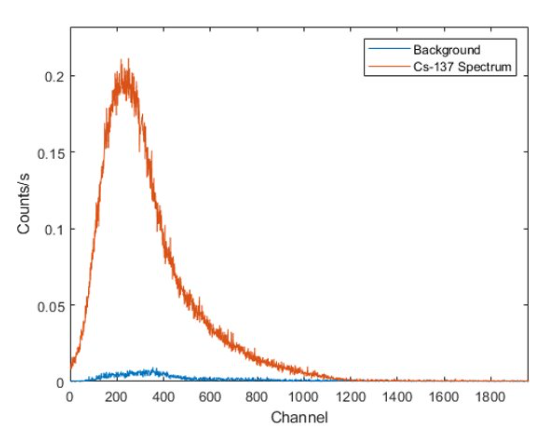
\includegraphics[width=0.80\textwidth]{figures/5_3_cspbbr_spectrum}
  \caption{Pulse-height spectrum acquired from the CsPbBr$_3$
           detector at 1000~V reverse bias with the $^{137}$Cs
           source present (solid line) and background-only
           (dashed line).  A clear elevation in total count rate
           is observed with the source, but no resolved photopeak
           is apparent due to the high electronic noise from the
           large device leakage current.  The anomalous feature
           near channel 16,382 is attributed to ADC saturation
           from ion-migration-induced current spikes.}
  \label{fig:cspbbr_spectrum}
\end{figure}

A Geant4 Monte Carlo simulation of the CsPbBr$_3$ crystal
geometry exposed to $^{137}$Cs (662-keV) gammas in a
$4\pi$ source configuration was performed to compute the
theoretical energy deposition spectrum.  The simulated
spectrum showed the characteristic features expected
for a small-volume Compton spectrometer: a Compton
continuum, a Compton edge, and a full-energy peak whose
intensity relative to the Compton continuum reflects
the small crystal volume and the resulting high
Compton-to-photoelectric ratio at 662~keV in a
medium-Z material.  Comparison of the simulated and
measured spectra confirmed that the measured spectrum
was dominated by electronic noise rather than any
intrinsic limitation of the CsPbBr$_3$ detector material:
the resolution-limiting factor was the large, unstable
leakage current and its noise contribution rather than
the charge transport properties of the crystal itself.

\subsection{FAPbBr$_3$ Gamma Spectroscopy}
\label{sec:fapbbr_gamma}

The FAPbBr$_3$ single-crystal detector, with a crystal
thickness of 2.35~mm and contact area of
$5.2 \times 6.15$~mm$^2$, demonstrated substantially
better high-voltage stability than the CsPbBr$_3$ device
and consequently produced more promising spectroscopic
results.  Electrical characterisation was first performed
with IV sweeps from $-20$ to $+20$~V and from $-200$ to
$+200$~V to assess the device leakage and confirm
acceptable Schottky behaviour.  A bias stability test
at $-200$~V over a six-hour period showed that the
leakage current reached a pseudo-steady-state with
a maximum measured value of $5 \pm 2.5$~nA during
high-voltage operation, approximately sixty times
lower than the CsPbBr$_3$ leakage at comparable bias.
The lower leakage in FAPbBr$_3$ at the same applied bias
is attributable to the better Schottky barrier quality
achieved with the Ti contact on this particular crystal,
which created a wider depletion region and a steeper
band-bending profile at the metal-semiconductor interface.

Spectroscopic measurements with $^{137}$Cs were
performed at bias voltages from 700~V upward, as shown
in Figure~\ref{fig:fapbbr_spectrum}.  At 700~V, the
spectrum showed a broad peak feature centred near the
expected channel position for the 662-keV photopeak,
with a count rate of approximately 17.45~counts\,s$^{-1}$
above a background of 9.11~counts\,s$^{-1}$.  At
1600~V bias, a simultaneous acquisition with both the
$^{137}$Cs (662-keV) and $^{57}$Co (122-keV) sources
produced a spectrum in which two distinct features could
be identified at channel positions consistent with the
expected photon energies when calibrated against a
reference CZT detector.  Figure~\ref{fig:fapbbr_spectrum}b
compares the $^{137}$Cs and $^{57}$Co spectra acquired
at 1600~V.  The count rates during acquisition were
9.11~counts\,s$^{-1}$ for background, 17.45~counts\,s$^{-1}$
for $^{137}$Cs, and 26.60~counts\,s$^{-1}$ for $^{57}$Co,
reflecting the higher specific activity of the $^{57}$Co
source used ($100~\mu$Ci vs.\ $5~\mu$Ci for $^{137}$Cs).

\begin{figure}[htbp]
  \centering
  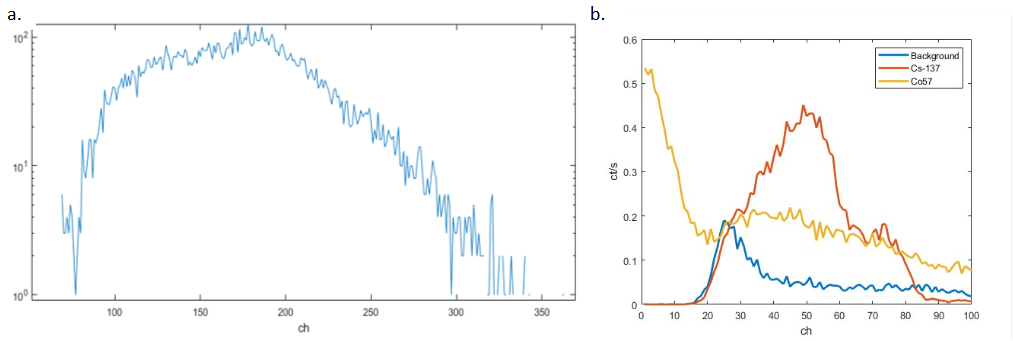
\includegraphics[width=0.85\textwidth]{figures/5_4_fapbbr_spectrum}
  \caption{(a) Pulse-height spectrum from the FAPbBr$_3$ detector
           under $^{137}$Cs irradiation at 700~V reverse bias,
           showing a broad peak feature near the expected
           photopeak channel.  (b) Spectrum comparison at 1600~V
           with $^{137}$Cs (5~$\mu$Ci) and $^{57}$Co (100~$\mu$Ci).
           Acquisition count rates: background 9.11~cps,
           $^{137}$Cs 17.45~cps, $^{57}$Co 26.60~cps.  The
           distinct features associated with each source's primary
           gamma energies can be resolved from the background
           continuum.}
  \label{fig:fapbbr_spectrum}
\end{figure}

While the FAPbBr$_3$ results represent a significant
improvement over the CsPbBr$_3$ device, the energy
resolution remains far below that required for
isotope identification in a practical nuclear security
application.  The resolution is limited by a combination
of factors: residual leakage-current noise even at the
low operating leakage of 5~nA; incomplete charge collection
arising from the carrier trapping described in
Section~\ref{sec:xray_trapping}; and ion
migration-induced fluctuations in the device's internal
electric field on timescales comparable to the spectroscopic
acquisition period, which cause the effective gain of the
detector to drift slowly and broaden any spectral features.

\subsection{MAPbBr$_3$ Fabrication Challenges}
\label{sec:mapbbr_issues}

The MAPbBr$_3$ crystal was processed through the same
pixelated Schottky contact fabrication protocol as the
other bromide systems, but failed to produce a
functional gamma spectrometer in the configuration
tested.  The primary cause was the poor quality of
the Ti Schottky contact achieved on this crystal.
The Ti deposition showed weak adhesion to the
polished MAPbBr$_3$ surface; upon venting the deposition
chamber to atmosphere, the Ti layer was observed to
partially delaminate, and subsequent IV characterisation
showed near-ohmic rather than Schottky behaviour.  This
outcome is attributed to two compounding factors.
First, the high sputter power used for Ti deposition
($\sim$450~W) produces fast-moving Ti adatoms with
high kinetic energies that may damage the soft perovskite
surface upon impact, creating a disordered interfacial
layer rather than a well-defined Schottky junction.
Literature on Ti Schottky contacts to halide perovskites
suggests that lower sputter power and higher chamber
vacuum produce higher barrier heights and improved
interface quality, a condition not satisfied with the
sputtering parameters used in this work~\cite{Saidaminov2015}.
Second, residual polishing compound at the crystal surface
— despite the hexane wash protocol — may have introduced
an insulating contamination layer that prevented intimate
metal-semiconductor contact.  As a consequence of the
failed Schottky barrier, the dark current in the
MAPbBr$_3$ device was too large to permit spectroscopic
measurements; the maximum usable bias before the
measurement was overwhelmed by noise was 20~V, at which
point the device had not yet entered a field regime
where charge collection efficiency was appreciable.


%% ------------------------------------------------------------
\section{Fast Neutron Detection}
\label{sec:neutron_detector}
%% ------------------------------------------------------------

\subsection{Motivation and Material Selection}
\label{sec:neutron_motivation}

Fast neutron detection poses a unique challenge because
neutrons carry no charge and therefore do not interact
directly with the electron clouds that govern the
response of conventional radiation detectors.  Instead,
fast neutrons must be detected indirectly by observing
the secondary charged particles — predominantly recoil
protons — produced in elastic scattering collisions with
hydrogen nuclei ($^1$H($n$,$n$)$^1$H).  The efficiency
of this conversion process is proportional to the
hydrogen number density $n_H$ of the detector material,
which for conventional hydrogenous semiconductors is
typically far too small to be competitive with
hydrogen-rich organic scintillators such as stilbene
or EJ-276 plastic.

MHyPbCl$_3$ was identified as a candidate fast neutron
semiconductor detector because its methylhydrazinium
cation (CH$_3$NH$_2$NH$_2^+$) contributes a substantial
number of hydrogen atoms per formula unit, giving a
calculated hydrogen density of approximately
$4.0 \times 10^{22}$~cm$^{-3}$ (Table~\ref{tab:h_density}),
comparable to stilbene ($5.67 \times 10^{22}$~cm$^{-3}$)
and rubrene ($3.62 \times 10^{22}$~cm$^{-3}$)~\cite{Panaccione_NIM_2024}.
Crucially, MHyPbCl$_3$ also exhibits the high resistivity
and large $\mu\tau$ product demonstrated in
Section~\ref{sec:electrical_char}, making it suitable
for direct charge-collection detection of the
recoil proton pulses generated by neutron scattering
events.  In this mode of operation, an individual
fast neutron interaction produces a recoil proton
of kinetic energy $E_p \leq E_n$ (the equality
holding for a head-on collision) that subsequently
deposits its energy entirely within the crystal,
generating an electron-hole pair population proportional
to $E_p / W$.  The resulting charge pulse is collected
by the applied field and read out by a charge-sensitive
preamplifier, enabling pulse-by-pulse energy analysis
and — in principle — reconstruction of the fast
neutron energy spectrum from the measured recoil
proton spectrum~\cite{Verbinski1968}.

An important complication for MHyPbCl$_3$ as a neutron
detector is the presence of lead in the crystal lattice.
With an atomic number of $Z = 82$, lead is a highly
efficient photon absorber via the photoelectric effect
at photon energies below its K-edge (88~keV) and
by Compton scattering at higher energies.  In a
mixed neutron-gamma radiation field such as that
produced by a research reactor, the detector therefore
responds to both neutrons and gammas simultaneously,
making clean separation of the two contributions
a significant analytical challenge.

\subsection{Fast Beam Facility and Beam Characterisation}
\label{sec:fbf_setup}

Neutron beam testing was performed at the Fast Beam
Facility (FBF) of the Ohio State University Research
Reactor (OSURR), a 500-kW$_{\rm th}$ pool-type research
reactor.  The FBF beamport incorporates a 4-inch
(10.16-cm) single-crystal bismuth gamma filter embedded
in the beam collimator assembly, which preferentially
attenuates the prompt reactor gamma flux while transmitting
fast neutrons.  A downstream 8-inch (20.32-cm) lead
gamma shutter — consisting of a cylindrical drum filled
with 1/16-inch Pb shot — can be inserted into the beam
path to provide an additional factor of
$\sim$300 in gamma reduction at the cost of a factor
of 58 in fast neutron attenuation.  An external 2-mm
cadmium (Cd) foil positioned at the beam exit port
can further reduce the thermal neutron content of the
beam; the Cd foil was characterised via gold foil
activation measurements per ASTM E262-17 to yield a
Cadmium Ratio of 1.1 and a thermal neutron reduction
factor of 110.

The neutron beam energy spectrum at the FBF, determined
by the SAND-II and STAYSL spectrum unfolding techniques
using activation of copper, gold, and nickel wire
dosimeters, is shown in Figure~\ref{fig:fbf_spectrum}.
The spectrum peaks in the fast neutron regime, with
a dominant fast neutron flux of approximately
$4.3 \times 10^5$~cm$^{-2}$\,s$^{-1}$ when the
gamma shutter is closed and no Cd filter is in place.
With the gamma shutter open and no Cd filter, the
fast neutron flux rises to
$1.5 \times 10^7$~cm$^{-2}$\,s$^{-1}$, accompanied
by a gamma dose rate of 15.787~R\,hr$^{-1}$ from
the prompt fission gamma field.  Insertion of the
lead gamma shutter reduces the gamma dose rate to
50.525~mR\,hr$^{-1}$ — a 300-fold reduction — while
attenuating the fast neutron flux by only a factor of
35 to $4.3 \times 10^5$~cm$^{-2}$\,s$^{-1}$.
Table~\ref{tab:fbf_conditions} summarises the beam
conditions used in this work.

\begin{table}[htbp]
\centering
\caption{FBF beam conditions used for MHyPbCl$_3$ neutron
         detection experiments.  All measurements at OSURR
         operating power.}
\label{tab:fbf_conditions}
\begin{tabular}{lcc}
\hline
Configuration & Fast Neutron Flux (cm$^{-2}$\,s$^{-1}$) & Gamma Dose Rate \\
\hline
Shutter open, no Cd   & $1.5\times10^7$ & 15.787~R\,hr$^{-1}$   \\
Shutter closed, no Cd & $4.3\times10^5$ & 50.525~mR\,hr$^{-1}$  \\
\hline
\end{tabular}
\end{table}

\begin{figure}[htbp]
  \centering
  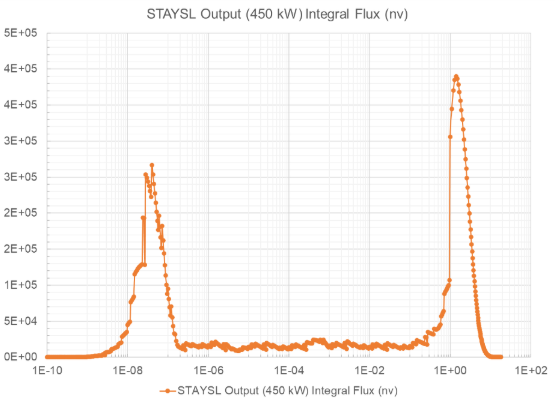
\includegraphics[width=0.70\textwidth]{figures/5_5_fbf_spectrum}
  \caption{Neutron energy spectrum at the OSURR Fast Beam
           Facility determined by SAND-II unfolding of
           Cu, Au, and Ni activation wire measurements.
           The spectrum is dominated by fast neutrons
           with energies from 0.1 to 10~MeV.}
  \label{fig:fbf_spectrum}
\end{figure}

Data were acquired using a CAEN A1422 charge-sensitive
preamplifier connected directly to the MHyPbCl$_3$
detector, with the preamplifier output recorded on a
Tektronix MSO54 oscilloscope in waveform-capture mode.
A Keithley 2612A SourceMeter provided the detector
bias voltage and simultaneously monitored the device
leakage current.  A cadmium foil chopper driven by a
motor was positioned in the beam path during selected
measurements to modulate the thermal neutron flux
periodically, enabling comparison of chopper-on
and chopper-off waveform populations.  The raw waveform
data were processed offline using a Python script that
applied a Locally Weighted Scatterplot Smoothing (LOWESS)
filter to suppress high-frequency electronic noise while
preserving the temporal profile of genuine
radiation-induced pulses.  Filtered waveforms were
then passed through a pulse-height analysis (PHA)
algorithm to reconstruct the energy deposition spectrum.

\subsection{Neutron Beam Test Results}
\label{sec:neutron_results}

The MHyPbCl$_3$ detector was operated at reverse bias
voltages of 80~V and 120~V for the FBF measurements.
Figure~\ref{fig:mhy_waveforms} shows representative
waveforms acquired from the preamplifier at 120~V
reverse bias with the gamma shutter open (mixed
neutron-gamma field) and with the gamma shutter closed
(fast neutron and residual gamma only).

\begin{figure}[htbp]
  \centering
  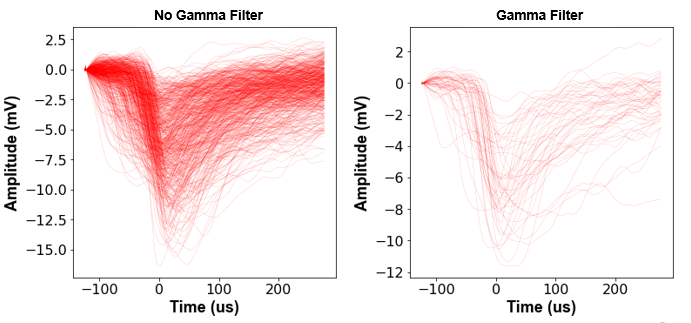
\includegraphics[width=0.85\textwidth]{figures/5_6_mhy_waveforms}
  \caption{Representative preamplifier waveforms from the
           MHyPbCl$_3$ detector at 120~V reverse bias at the
           OSURR FBF.  (a) Gamma shutter open (mixed field).
           (b) Gamma shutter closed (reduced gamma, fast
           neutron dominant).  (c) Beam background acquired
           in the shutter-closed configuration with the
           reactor at power.  Radiation-induced pulses are
           visible above the noise floor in all three
           configurations.}
  \label{fig:mhy_waveforms}
\end{figure}

At 120~V reverse bias with the gamma shutter open,
1090 waveforms containing radiation-induced pulses were
collected over the acquisition interval.  After closing
the gamma shutter, 1001 pulses were recorded over a
comparable interval; the beam background (reactor at
power, beam blocked entirely) yielded 394 pulses.
The count rate with the shutter closed
($\sim$0.5~counts\,s$^{-1}$) was not meaningfully
different from the shutter-open count rate at 120~V
in the forward bias configuration (Figure~\ref{fig:mhy_forward}),
a result that is discussed further in
Section~\ref{sec:neutron_discussion} below.

At 80~V reverse bias, the total waveform counts with the
gamma shutter open were 1040 (shutter open) and 507
(shutter closed) versus 252 for background.  The
ratio of source-to-background counts at 80~V is higher
than at 120~V, suggesting that the lower field at 80~V
produces a different carrier collection regime in which
the relative contribution of high-charge-deposition
events (which would include both neutron proton-recoil
events and direct gamma interactions) is more clearly
separated from the background noise floor.

Pulse height analysis of the filtered waveforms at
120~V reverse bias is shown in Figure~\ref{fig:mhy_pha}.
The resulting spectrum does not display a sharp Gaussian
peak indicative of full-energy deposition from a
mono-energetic source; rather, it exhibits a broad
continuum of pulse heights extending from the noise
threshold to the maximum digitised amplitude.  This
spectral shape is physically expected for fast neutron
detection: recoil protons from elastic scattering of
poly-energetic fast neutrons produce a broad energy
deposition distribution, and the convolution of this
distribution with the incomplete charge collection at
the bias voltages used here further broadens the
response.  Nevertheless, the waveform population
is clearly distinct from the background (reactor off)
waveform population, confirming that the MHyPbCl$_3$
crystal is responding to radiation from the reactor
beam.

\begin{figure}[htbp]
  \centering
  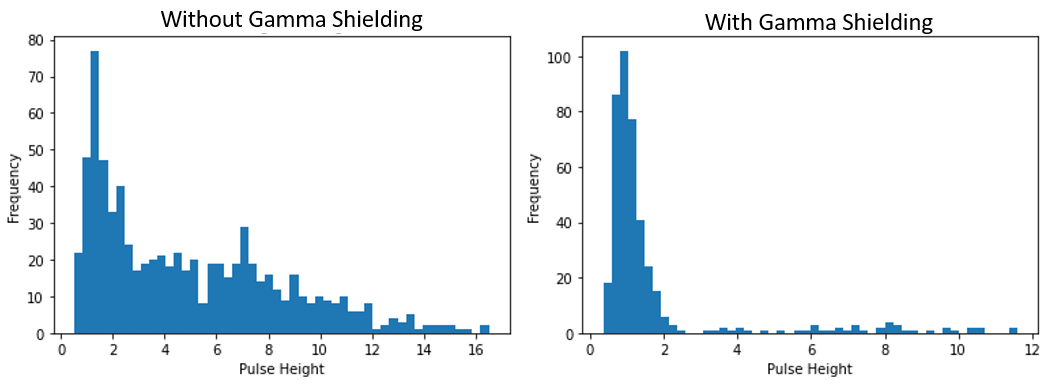
\includegraphics[width=0.75\textwidth]{figures/5_7_mhy_pha}
  \caption{Pulse-height spectrum reconstructed from LOWESS-filtered
           waveforms from the MHyPbCl$_3$ detector at 120~V
           reverse bias.  (a) No gamma filter applied (mixed field).
           (b) Gamma shutter closed.  The broad continuum is
           consistent with the expected proton-recoil energy
           deposition spectrum from a poly-energetic fast
           neutron beam.}
  \label{fig:mhy_pha}
\end{figure}

\subsection{Neutron-Gamma Discrimination and Detection Efficiency}
\label{sec:neutron_discussion}

The neutron-gamma discrimination challenge is illustrated
by the comparison between shutter-open and shutter-closed
waveform populations.  When the lead gamma shutter is
closed, the gamma dose rate is reduced by a factor of
approximately 300 (from 15.787~R\,hr$^{-1}$ to
50.525~mR\,hr$^{-1}$), while the fast neutron flux
decreases by only a factor of 35.  If the detector
were responding purely to neutrons, one would expect
the pulse count rate with the shutter closed to be
approximately $35/300 \approx 0.12$ times the
shutter-open count rate.  The observed shutter-open
to shutter-closed count rate ratio at 120~V reverse
bias (1090:1001, after background subtraction) does
not show this level of suppression.  The most likely
interpretation is that the detector response at
120~V bias is dominated by direct gamma interactions
(via Compton scattering and photoelectric absorption
in the Pb sublattice) rather than neutron-induced
proton recoil events.  This result highlights the
fundamental difficulty of neutron-gamma discrimination
in a Pb-containing semiconductor: the heavy Pb sublattice
that makes the material mechanically robust and
electrically well-behaved also makes it an efficient
gamma absorber that overwhelms the neutron-induced signal
in mixed radiation fields.

An upper bound estimate of the intrinsic detection
efficiency for fast neutrons in the MHyPbCl$_3$ crystal
can be computed from the hydrogen density, the crystal
dimensions, and the elastic scattering cross section.
At a neutron energy of 1~MeV, the $^1$H($n$,$n$)$^1$H
elastic cross section is approximately 3~b~\cite{ENDF8}.
For a crystal with an effective thickness of 5~mm
normal to the beam and a hydrogen density of
$4.0 \times 10^{22}$~cm$^{-3}$, the interaction
probability per incident neutron is

\begin{equation}
  P = 1 - \exp(-n_H \sigma_{\rm el} t)
    \approx 1 - \exp(-4.0\times10^{22} \times 3\times10^{-24}
             \times 0.5)
    \approx 5.8\%,
  \label{eq:neutron_eff}
\end{equation}

\noindent where $t = 0.5$~cm is the path length.  At the
fast neutron flux of $4.3 \times 10^5$~cm$^{-2}$\,s$^{-1}$
(shutter closed) and the $\sim$0.3-cm$^2$ detector area,
this implies an expected proton-recoil interaction rate
of $\sim$750~events per second — far larger than the
0.5~counts\,s$^{-1}$ actually observed.  The discrepancy
is explained primarily by the oscilloscope waveform-write-rate
bottleneck: the Tektronix MSO54 oscilloscope in
single-shot waveform acquisition mode is capable of
writing at a maximum rate that was the dominant constraint
on the measurable count rate in this configuration.
Increasing the data acquisition throughput — for example
by switching to a hardware MCA or a fast digitiser in
continuous acquisition mode — is the highest-priority
hardware improvement identified for future neutron
detection experiments.


%% ------------------------------------------------------------
\section{Ion Migration and Device Stability}
\label{sec:ion_migration_detector}
%% ------------------------------------------------------------

The experimental results presented in Sections~\ref{sec:xray_detector}
through~\ref{sec:neutron_detector} are pervaded by a single
overarching materials-physics challenge: the migration of halide
ions under the large applied electric fields required for
efficient charge collection.  Ion migration is not unique to
the detector geometry; as noted in Chapter~\ref{ch:CsFAPbI},
it also affects the photovoltaic devices studied in that chapter
under their built-in fields.  However, the detector geometry
exacerbates the problem in two important ways.  First, the
fields required for efficient charge collection ($\sim$1~V~$\mu$m$^{-1}$
across millimetre-scale crystals) are several orders of
magnitude larger than the built-in fields in a photovoltaic
device.  Second, the crystal must sustain these fields
continuously for hours at a time during a spectroscopy
acquisition, rather than the millisecond timescales over
which a radiation monitoring current measurement is averaged.
The combination of large field and long exposure duration
creates an environment in which ion migration is not merely
a nuisance but a device-lifetime-limiting degradation mechanism.

\subsection{Humidity-Dependent Instability}
\label{sec:humidity_instability}

A systematic investigation of the relationship between
ambient humidity and device stability in 2D perovskite
(PEA$_2$MA$_2$Pb$_3$I$_{10}$) detectors, performed by
Tsai et al.\ and reported in part here due to the direct
co-investigator contribution of this work, established
that the severity of voltage-induced instability is
directly correlated with the relative humidity (RH) of
the operating environment~\cite{Tsai2022ionmig}.  In
those experiments, devices with the p-i-n architecture
(PTAA / 2D perovskite / C$_{60}$:BCP / Au) were subjected
to IV sweeps and bias-hold tests at controlled RH levels
of 0\%, 20\%, and 40\% in a sealed chamber.

At 0\% RH (inert atmosphere), the devices exhibited
no measurable I-V hysteresis across the tested voltage
range and remained stable under sustained reverse bias
to voltages beyond $-15$~V.  As the RH was raised to
20\% and then to 40\%, the hysteresis in the forward-to-reverse
sweep became progressively more pronounced, and the
breakdown voltage decreased dramatically: devices at
40\% RH failed irreversibly at bias voltages as low as
$-8$ to $-10$~V, whereas their counterparts tested at
0\% RH survived to voltages more than twice as large.
Time-resolved dark current measurements at constant
$-5$~V bias in 40\% RH air showed that devices failed
within two to three minutes, while the same devices
at zero bias in 40\% RH remained stable for over
one hour.

The mechanism by which humidity accelerates
voltage-induced breakdown was identified through
a combination of photoluminescence (PL) mapping
and quantum chemical simulations~\cite{Tsai2022ionmig}.
PL peak-position maps acquired after voltage stressing
at $-1$, $-5$, and $-7$~V showed that the unprotected
device developed pronounced spatial inhomogeneity in
its PL wavelength and intensity after $-7$~V stress,
with local ``hot spots'' of shifted emission indicative
of ion-migration-driven phase segregation.  In contrast,
devices treated with a 4-mg\,mL$^{-1}$ coating of
5-fluorinated phenylethylammonium iodide (5F-PEAI) on
the perovskite surface showed PL distributions that
were essentially unchanged after identical voltage stress.
DFT calculations of the water migration pathway through
the PEA and 5F-PEA organic layers revealed a key mechanistic
difference: the activation energy for water diffusion
through the PEA layer is only $\sim$5~meV, far below
the thermal energy at room temperature, meaning that
water molecules penetrate through the organic capping
layer to the inorganic Pb-I framework essentially without
barrier.  In contrast, the fluorinated 5F-PEA layer
raised the activation barrier for water penetration
to $\sim$120~meV, an energy comparable to $k_BT$
at elevated temperatures and sufficient to significantly
retard moisture ingress under ambient conditions.

These mechanistic findings directly inform the
observations made in this work.  The CsPbBr$_3$
detector's long leakage-current stabilisation time
(45 minutes to one hour at 1000~V bias) and the
MAPbI$_3$-hBN device's catastrophic failure at 400~V
after five hours are both consistent with the
moisture-accelerated ion-migration mechanism.  The
vacuum test results (Section~\ref{sec:vacuum_testing})
confirm this: removing moisture from the environment
by operating under vacuum substantially reduced the
leakage current and delayed failure, directly
analogous to the 0\% RH inert atmosphere experiments
in the Tsai et al.\ study.

\subsection{Contact Degradation at Elevated Bias}
\label{sec:contact_degradation}

A second and distinct degradation mechanism was identified
during testing of the FAPbBr$_3$ device: the chemical
reaction of the titanium Schottky contact with mobile
bromide ions generated and driven toward the contact
interface under the large applied reverse bias.  After
a full day of electrical testing at the Ti1 contact
of the FAPbBr$_3$ crystal, the contact surface was
visually observed to have changed colour and the
metallic titanium layer appeared to have partially
receded into or reacted with the perovskite crystal
surface.  Elemental analysis of the relevant ionic
species identifies the reaction as plausible: mobile
bromide ions (charge $-1$) accumulating at the Ti
contact (Ti in the $+3$ oxidation state in many
common compounds) can form stable titanium bromide
complexes (e.g.\ TiBr$_4^{2-}$), consuming the metal
electrode.  The relevant charge states of the species
present — Br$^-$, Ti$^{3+}$, Pb$^{2+}$, and the
organic FA$^+$ cation — are all present at the
interface under the reverse-bias condition that
drives Br$^-$ toward the titanium contact.

This failure mode has profound implications for contact
material selection in bromide perovskite radiation
detectors.  Metals that form stable halide compounds
under the electrochemical conditions encountered at
the reversed-biased contact — titanium being one
such metal — are fundamentally incompatible with
sustained high-field operation in halide perovskite
detectors, regardless of their electronic Schottky
barrier properties.  Gold, by contrast, forms only
kinetically stable halide compounds under mild
conditions and showed no evidence of analogous
chemical degradation at the ohmic contact in any
device examined in this work.  Alternative
contact materials identified in the broader
perovskite detector literature as candidates for
improved chemical stability include chromium
(Cr) and tin oxide (SnO$_2$), both of which were
evaluated on the CsPbBr$_3$ crystal at the
Cr/SnO$_2$/Cr contact in preliminary experiments;
however, these contacts were not carried through
to full spectroscopic evaluation within the scope
of this work.

\subsection{Ion Migration Consequences for Spectroscopy}
\label{sec:ion_migration_spectroscopy}

Beyond the acute failure modes described above, ion
migration impairs spectroscopic performance through
three mechanisms that together set a practical upper
bound on the achievable energy resolution in
as-fabricated perovskite single crystal detectors.

First, the redistribution of ions under the applied
field creates a non-uniform internal electric field
profile.  In an ideal crystal with uniform space charge,
the electric field is constant across the bulk between
the contacts.  As mobile anions accumulate at the
anode and cations at the cathode, a positive space-charge
layer forms near the cathode and a negative space-charge
layer near the anode.  This space charge creates an
opposing electric field that adds to the applied field
at one interface and subtracts from it at the other,
producing a spatially non-uniform field profile in the
bulk.  Carriers generated at different depths in the
crystal therefore experience different net fields and
have different collection probabilities, broadening
the pulse-height distribution for monoenergetic
radiation events and degrading the achievable energy
resolution~\cite{He1997CZT}.

Second, the current overshoot observed upon initial
application of bias — where the leakage current
transiently rises above its quasi-steady-state value
before decaying over tens of minutes — causes the
internal field distribution to evolve continuously
during the acquisition.  Since the peak position in
a pulse-height spectrum is proportional to the
instantaneous charge collection efficiency (which in
turn depends on the internal field profile), the
slow time evolution of the field distribution during
ion migration causes the effective detector gain to
drift, further broadening accumulated spectral peaks.

Third, on long timescales, the accumulated ionic charge
at the interfaces depresses the net electric field
in the bulk, reducing the drift velocity of radiation-generated
carriers and increasing the probability of trapping
before collection — the same trapping mechanism
identified in Section~\ref{sec:xray_trapping}
for X-ray sensitivity degradation.  The combination
of these three effects means that the energy resolution
of a perovskite detector operated at high bias in
ambient conditions will inevitably worsen over time,
even if the initial resolution at the moment of bias
application is acceptable.

\subsection{Mitigation Strategies}
\label{sec:mitigation}

Several mitigation strategies were evaluated or
identified in the course of this work.  Vacuum operation
was demonstrated to extend the operational lifetime
of the MAPbI$_3$-hBN device and to improve X-ray
sensitivity at matched bias voltages.  However, vacuum
operation is impractical for most field applications
of radiation detectors, and it addresses only the
humidity-acceleration pathway rather than the
intrinsic ion-migration driving force provided by
the applied electric field.

Surface passivation with 5F-PEAI, demonstrated by
Tsai et al.\ in 2D perovskite detectors, represents
a more promising approach for thin-film device
geometries.  At a concentration of 4~mg\,mL$^{-1}$,
5F-PEAI penetrates the grain boundaries of the
perovskite film (as confirmed by ToF-SIMS fluorine
mapping) and raises the water-penetration activation
energy sufficiently to stabilise the device to $-16$~V
in 40\% RH air, compared to $-10$~V for the
unprotected device.  The sensitivity of the
5F-PEAI-protected device approached
$996~\mu$C\,(Gy$_{\rm air}$\,cm$^2$)$^{-1}$ at
4~V bias — among the highest reported for polycrystalline
perovskite detectors of comparable thickness.
Extending this passivation strategy to the 3D single
crystal systems examined in this work is identified
as a high-priority direction for future research.

Contact material engineering is a second avenue
for mitigating contact-specific degradation.  The
chemical reaction of Ti contacts with mobile Br$^-$
ions — documented here for the first time in the
context of perovskite radiation detectors — motivates
the replacement of Ti with contact metals that do
not form stable halide compounds, such as Au
(already used on the ohmic side), Pt, or Cr-based
multilayers.  Independently, the use of
carrier-selective interlayers (such as the C$_{60}$:BCP
bilayer used in the MHyPbCl$_3$ device) both at
the Schottky and ohmic contacts can reduce the
effective recombination velocity at the interfaces
and thereby extend the field range over which stable
detector operation is achievable.

A third mitigation approach is improved crystal quality
— specifically, the reduction of halide vacancy
concentrations that provide the mobile ionic carriers.
Growth conditions that minimise the stoichiometric
excess of either the organic cation or the lead halide
precursor, such as the slow anti-solvent crystallisation
used for MHyPbCl$_3$, or the use of single-crystal
growth methods under inert atmosphere, have been shown
to produce lower intrinsic defect densities and
improved electrical stability in the photovoltaic
literature~\cite{Saidaminov2015}.  Applying these
best-practice growth conditions systematically to
the detector crystal geometries required here is
an important near-term research goal.


%% ------------------------------------------------------------
\section{Summary}
\label{sec:ch5_summary}
%% ------------------------------------------------------------

This chapter has described the development and characterisation
of halide perovskite direct-conversion radiation detectors
for three distinct radiation types: X-rays, gamma rays, and
fast neutrons.

For X-ray detection, the MAPbI$_3$-hBN device demonstrated
a monotonically increasing sensitivity with applied bias:
$0.107$, $0.245$, and $0.411~\mu$C\,(Gy\,cm$^2$)$^{-1}$
at 5, 10, and 20~V, respectively, consistent with the
Hecht equation prediction for improving charge collection
at higher fields.  Vacuum testing confirmed that the removal
of ambient moisture enhanced both sensitivity and stability,
directly attributing the performance degradation observed
in ambient air to moisture-accelerated ion migration.
The device failed irreversibly after approximately five
hours at 400~V, setting an empirical upper bound on the
sustainable bias for this material-contact combination
in the absence of surface passivation.

For gamma-ray detection, three bromide perovskite systems
were evaluated.  The CsPbBr$_3$ device produced a
statistically significant count-rate response to a
$^{137}$Cs source (17.45~cps vs.\ 9.11~cps background)
at 1000~V bias, but the high and unstable leakage current
(315--710~nA) generated electronic noise that prevented
resolution of the 662-keV photopeak.  The FAPbBr$_3$
device, which achieved substantially lower operating
leakage ($5 \pm 2.5$~nA maximum at high bias) and sustained
stable high-voltage operation for over five hours, produced
spectral features attributable to both $^{137}$Cs and
$^{57}$Co in a joint acquisition at 1600~V bias, representing
a proof-of-concept demonstration of gamma spectroscopy in
a solution-grown halide perovskite crystal.  The MAPbBr$_3$
device failed to produce functional Schottky contacts under
the deposition conditions used, due to high sputter power
and surface contamination from polishing, motivating a
revised contact deposition protocol at reduced sputter power.

For fast neutron detection, MHyPbCl$_3$ crystals were
characterised as the first organic-metal halide
perovskite semiconductor evaluated in a reactor fast
neutron beam.  The material combines a high hydrogen
density ($\sim 4.0 \times 10^{22}$~cm$^{-3}$, comparable
to stilbene) with an exceptional resistivity of
$4.43 \times 10^{11}$~$\Omega$\,cm and a $\mu\tau$ product
of $9.1 \times 10^{-3}$~cm$^2$\,V$^{-1}$.  Waveform
data acquired at the OSURR FBF confirmed radiation-induced
pulse activity distinct from the beam background, and
pulse-height analysis produced spectra consistent with
the expected broad proton-recoil energy deposition
distribution from a poly-energetic fast neutron beam.
Neutron-gamma discrimination remains a challenge due to
the large Pb content of MHyPbCl$_3$, and the data
acquisition bottleneck imposed by the oscilloscope
waveform write rate prevented collection of sufficient
statistics for quantitative efficiency analysis.

Across all three detection modes, ion migration under
applied electric fields emerged as the central
performance-limiting mechanism.  The correlation of
device instability with ambient humidity — confirmed
both by the vacuum tests on MAPbI$_3$-hBN and by
the systematic humidity-dependence study on 2D perovskite
detectors — points to surface passivation, such as the
5F-PEAI treatment demonstrated to produce sensitivities
approaching $\sim$1000~$\mu$C\,(Gy$_{\rm air}$\,cm$^2$)$^{-1}$
in thin-film detectors, as the most promising near-term
strategy for extending the operational stability of
perovskite radiation detectors toward the performance
levels required for practical deployment.